%% LyX 2.0.6 created this file.  For more info, see http://www.lyx.org/.
%% Do not edit unless you really know what you are doing.
\documentclass[english]{article}
\usepackage[T1]{fontenc}
\usepackage[latin9]{inputenc}
\usepackage{units}
\usepackage{textcomp}
\usepackage{amsmath}
\usepackage{graphicx}
\usepackage{esint}

\makeatletter

%%%%%%%%%%%%%%%%%%%%%%%%%%%%%% LyX specific LaTeX commands.
%% Because html converters don't know tabularnewline
\providecommand{\tabularnewline}{\\}

\makeatother

\usepackage{babel}
\begin{document}

\title{Modelling airfoil flaps with an orthogonal curvilinear coordinate
transformation}


\author{Gael de Oliveira}

\maketitle
\vphantom{}\vphantom{}\vphantom{}\vphantom{}\vphantom{}\vphantom{}\vphantom{}\vphantom{}\vphantom{}\vphantom{}\vphantom{}\vphantom{}\vphantom{}\vphantom{}\vphantom{}
\begin{abstract}
We follow Goldstein (1938) in our exploration of Lam�'s (1859) formidable
work on curvilinear coordinate systems to define an conformal (angle-preserving)
airfoil transformation parametrized by an arbitrary chordline deformation
interpolant. There is nothing fundamentally new in this work, but
the author hopes this piece will serve as advocacy material for the
formidable potential of orthogonal curvilinear coordinate tranformations.

We propose an hybrid analytical-numerical implementation which works
as a prototyping code to support many of our short term activities:
continuous flap modelling for VI-code (e.g. R/Xfoil) analysis and
airfoil optimization, generation of equivalent shapes to account for
inhomogeneous inflow cases in standard panel codes (e.g. curved inflow
in a VAWT case), thin mesh generation and deformation for hybrid Lagrangian-Eulerian
approaches (e.g. PhyFLOW) or dynamic differential operator modification
in ALE FV codes applied to fluid-structure interaction (in the longer
term!).
\end{abstract}
\pagebreak{}

\vphantom{}\vphantom{}\vphantom{}\vphantom{}\vphantom{}\vphantom{}\vphantom{}\vphantom{}\vphantom{}\vphantom{}\vphantom{}\vphantom{}\vphantom{}\vphantom{}\vphantom{}\vphantom{}\vphantom{}\vphantom{}\vphantom{}\vphantom{}\vphantom{}\vphantom{}

\tableofcontents{}

\pagebreak{}


\section{Flap rotation}


\subsection{Hinge line deformation }


\subsubsection{Solid Body Rotation}

Consider a flap rotated as a rigid body by an angle $\theta$ around
its hinge. The deformed hinge line will be given as a piecewise linear
function inflected at the hinge position $x_{h}$:

\[
f_{\left(x\right)}=\begin{cases}
c & \quad,\quad0<x<x_{h}\\
c+m\left(x-x_{hinge}\right) & \quad,\quad x_{h}\leq x
\end{cases}
\]


where $m$ is the slope of the deformed hinge line, directly related
to the flap angle $\theta$: 
\[
m=\tan\theta
\]


and the first derivative of the hinge line will written:
\[
\frac{df}{dx}=\begin{cases}
0 & \quad,\quad x<x_{hinge}\\
m & \quad,\quad x\geq x_{hinge}
\end{cases}
\]


clearly showing that the \textquotedbl{}pure\textquotedbl{} solid
body rotation introduces a first derivative discontinuity, and hence
a ``corner'' in the hinge line.


\subsubsection{Smoothing Solid Body Rotation}

To eliminate $1^{st}$ derivative discontinuities we will start by
developping a softened , $C^{2}$ continuous form of the hingeline
deformation function $f$ whose softness will depend on a knee parameter$\delta$:
\[
f_{\left(x\right)}=\begin{cases}
c & \quad,\quad x<x_{h}-\delta\\
p_{\left(x\right)} & \quad,\quad x_{h}-\delta\leq x<x_{h}+\delta\\
c+m\left(x-x_{h}\right) & \quad,\quad x_{h}+\delta\leq x
\end{cases}
\]


and $p_{\left(x\right)}$ will be chosen to be a smooth function such
that $f$ preserves $C^{2}$ continuity. For this purpose, we set
that $p_{\left(x\right)}$ will abide to the following boundary conditions:

\begin{table}[h]
\begin{centering}
\begin{tabular}{|c|c|c|c|}
\hline 
$x$ & $p$ & $\frac{dp}{dx}$ & $\frac{d\text{\texttwosuperior}p}{dx\text{\texttwosuperior}}$\tabularnewline
\hline 
\hline 
$x_{h}-\delta$ & $c$ & 0 & $0$\tabularnewline
\hline 
$x_{h}+\delta$ & $c+m\delta$ & $m$ & $0$\tabularnewline
\hline 
\end{tabular}
\par\end{centering}

\caption{g-eta-x function boundary conditions}
\end{table}



\subsubsection{Looking for a C2-smooth knee function}

The $p$ function can also be written in terms of a $C^{2}$ smooth
function $g$, a scaling $\delta m$, and a coordinate tranformation
$\eta_{\left(x\right)}$ 
\[
p_{\left(x\right)}=2\delta mg_{\left(\eta_{\left(x\right)}\right)}+c
\]


with the coordinate transformation $\eta_{\left(x\right)}$ defined
as:
\[
\eta_{\left(x\right)}=\frac{x-\left(x_{h}-\delta\right)}{\left(x_{h}+\delta\right)-\left(x_{h}-\delta\right)}=\frac{x-x_{h}}{2\delta}+\frac{1}{2}
\]


in which case the boundary conditions can be restated as:

\begin{table}[h]
\begin{centering}
\begin{tabular}{|c|c|c|c|c|}
\hline 
$x$ & $\eta$ & $g$ & $\frac{\partial g}{\partial\eta}$ & $\frac{\partial^{2}g}{\partial\eta^{2}}$\tabularnewline
\hline 
\hline 
$x_{h}-\delta$ & $0$ & $0$ & $0$ & $0$\tabularnewline
\hline 
$x_{h}+\delta$ & $1$ & $\frac{1}{2}$ & $1$ & $0$\tabularnewline
\hline 
\end{tabular}
\par\end{centering}

\caption{g-eta-x function boundary conditions}
\end{table}


Considering these boundary conditions, we decide to look for a suitable
expression for $g$ in the form a polynomial%
\footnote{Other forms could also be chosen: trigonometric function series, exponentials,
and many others. But my intuition tells me polynomials are usually
a good starting point for this sort of problems!%
}. The 6 boundary conditions produce 6 equations binding the $g$ function,
and so, assuming the conditions are independent, there will be one
and only on 6th order, 5th degree, polynomial satisfying all six boundary
conditions. 

\begin{figure}
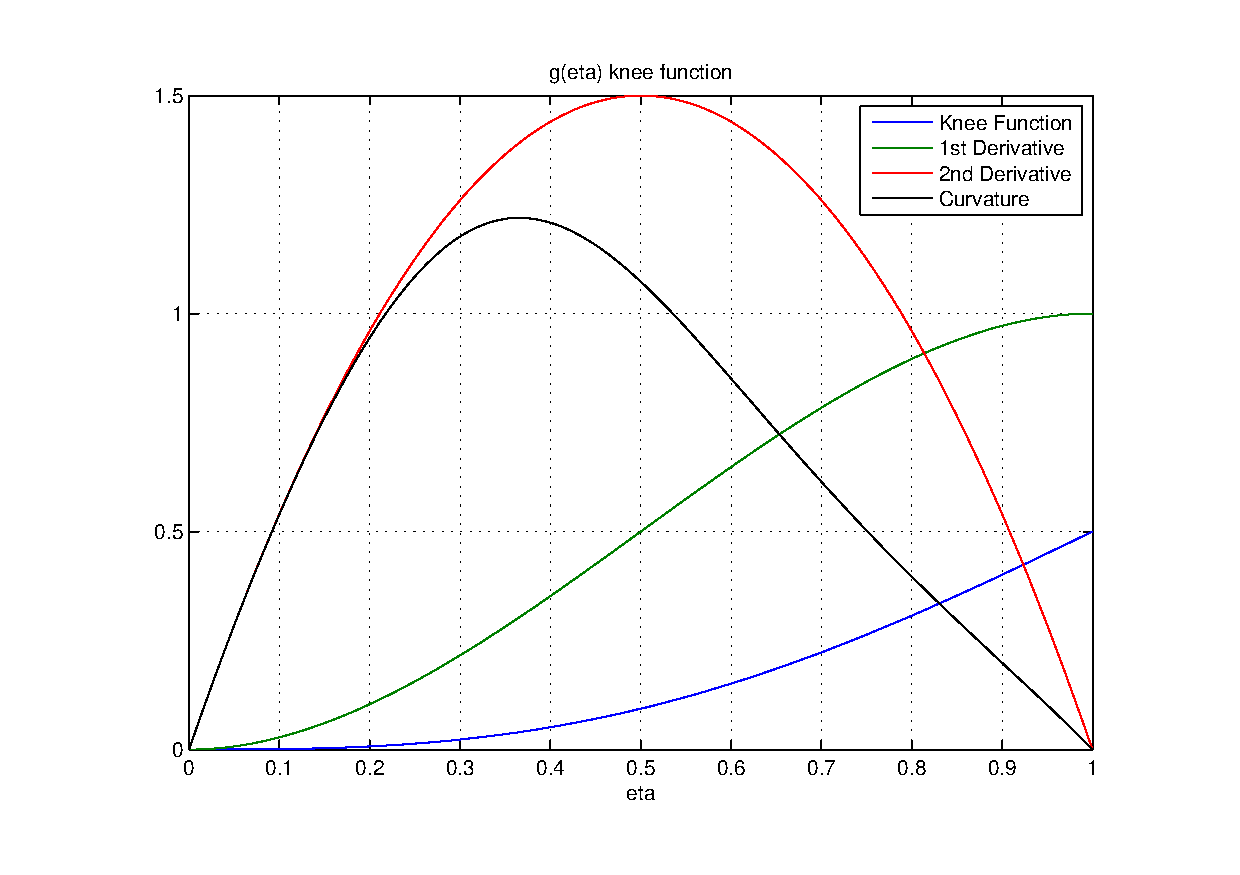
\includegraphics[width=0.9\textwidth]{fig/scaled_knee_function}

\caption{The g-eta knee function}
\end{figure}


To look for that polynomial, we will first write it as a dot product
between its six coefficients and the canonical polynomial base elements:
\[
g_{\left(\eta\right)}=\sum_{i=0}^{5}a_{i}\eta^{i}=\left[\begin{array}{cccccc}
1 & \eta & \eta^{2} & \eta^{3} & \eta^{4} & \eta^{5}\end{array}\right]\left[\begin{array}{c}
a_{0}\\
a_{1}\\
a_{2}\\
a_{3}\\
a_{4}\\
a_{5}
\end{array}\right]
\]


We can now write the $1^{st}$ and $2^{nd}$ derivatives of $g$ in
a similar form:
\[
\frac{\partial g}{\partial\eta}=\frac{\partial}{\partial\eta}\left(\sum_{i=0}^{5}a_{i}\eta^{i}\right)=\sum_{i=0}^{5}a_{i}\frac{\partial}{\partial\eta}\left(\eta^{i}\right)=\left[\begin{array}{cccccc}
0 & 1 & 2\eta & 3\eta^{2} & 4\eta^{3} & 5\eta^{4}\end{array}\right]\left[\begin{array}{c}
a_{0}\\
a_{1}\\
a_{2}\\
a_{3}\\
a_{4}\\
a_{5}
\end{array}\right]
\]
\[
\frac{\partial^{2}g_{\left(\eta\right)}}{\partial\eta^{2}}=\sum_{i=0}^{5}a_{i}\frac{\partial^{2}}{\partial\eta^{2}}\left(\eta^{i}\right)=\left[\begin{array}{cccccc}
0 & 0 & 2 & 6\eta & 12\eta^{2} & 20\eta^{3}\end{array}\right]\left[\begin{array}{c}
a_{0}\\
a_{1}\\
a_{2}\\
a_{3}\\
a_{4}\\
a_{5}
\end{array}\right]
\]


providing us for a straightforward way to write a linear system :
\[
\left[\begin{array}{c}
\left[g_{\left(\eta=0\right)}\right]\\
\left[\frac{\partial g}{\partial\eta}_{\left(\eta=0\right)}\right]\\
\left[\frac{\partial^{2}g}{\partial\eta^{2}}_{\left(\eta=0\right)}\right]\\
\left[g_{\left(\eta=1\right)}\right]\\
\left[\frac{\partial g}{\partial\eta}_{\left(\eta=1\right)}\right]\\
\left[\frac{\partial^{2}g}{\partial\eta^{2}}_{\left(\eta=1\right)}\right]
\end{array}\right]=\left[\begin{array}{c}
0\\
0\\
0\\
\nicefrac{1}{2}\\
1\\
0
\end{array}\right]
\]


and  express it in matrix form in terms of the coefficients: 
\[
\left[M\right]\left\{ A\right\} =\left\{ B\right\} \qquad\Leftrightarrow\qquad\left[\begin{array}{cccccc}
1 & 0 & 0 & 0 & 0 & 0\\
0 & 1 & 0 & 0 & 0 & 0\\
0 & 0 & 2 & 0 & 0 & 0\\
1 & 1 & 1 & 1 & 1 & 1\\
0 & 1 & 2 & 3 & 4 & 5\\
0 & 0 & 2 & 6 & 12 & 20
\end{array}\right]\left[\begin{array}{c}
a_{0}\\
a_{1}\\
a_{2}\\
a_{3}\\
a_{4}\\
a_{5}
\end{array}\right]=\left[\begin{array}{c}
0\\
0\\
0\\
\nicefrac{1}{2}\\
1\\
0
\end{array}\right]
\]


Fortunately, the matrix has rank 6, and this means that:
\begin{enumerate}
\item The boundary conditions are indeed independent from each other
\item The matrix is invertible and the linear system has a unique solution
\end{enumerate}
The solution is obtained by inverting the matrix numerically%
\footnote{Manual gaussian elimination would also work on this system!%
}, and has a very clean form:

\[
\left[\begin{array}{c}
a_{0}\\
a_{1}\\
a_{2}\\
a_{3}\\
a_{4}\\
a_{5}
\end{array}\right]=\left[\begin{array}{c}
0\\
0\\
0\\
1\\
-\nicefrac{1}{2}\\
0
\end{array}\right]
\]


We can write the $g$ function and its derivatives explicitly as:
\[
g_{\left(\eta\right)}=\eta^{3}-\frac{\eta^{4}}{2}\qquad,\qquad\frac{\partial g}{\partial\eta}=3\eta^{2}-2\eta^{3}\qquad,\qquad\frac{\partial^{2}g}{\partial\eta^{2}}=6\eta-6\eta^{2}
\]


So that the curvature of the $g-\eta$'s graphline is written as:
\[
\kappa_{g}=\frac{\frac{\partial^{2}g}{\partial\eta^{2}}}{\left(1+\left(\frac{\partial g}{\partial\eta}\right)^{2}\right)^{\frac{3}{2}}}=\frac{6\eta-6\eta^{2}}{\left(\left(3\eta^{2}-2\eta^{3}\right)^{2}+1\right)^{\frac{3}{2}}}
\]


for which there exists an analytical primitive in $\eta$:
\[
\int\kappa_{g}d\eta=\frac{\left(3\eta^{2}-2\eta^{3}\right)\sqrt{\left(3\eta^{2}-2\eta^{3}\right)^{2}+1}}{4\eta^{6}-12\eta^{5}+9\eta^{4}+1}
\]


which will facilitate the construction of an orthogonal curvilinear
coordinate transformation.

\begin{figure}
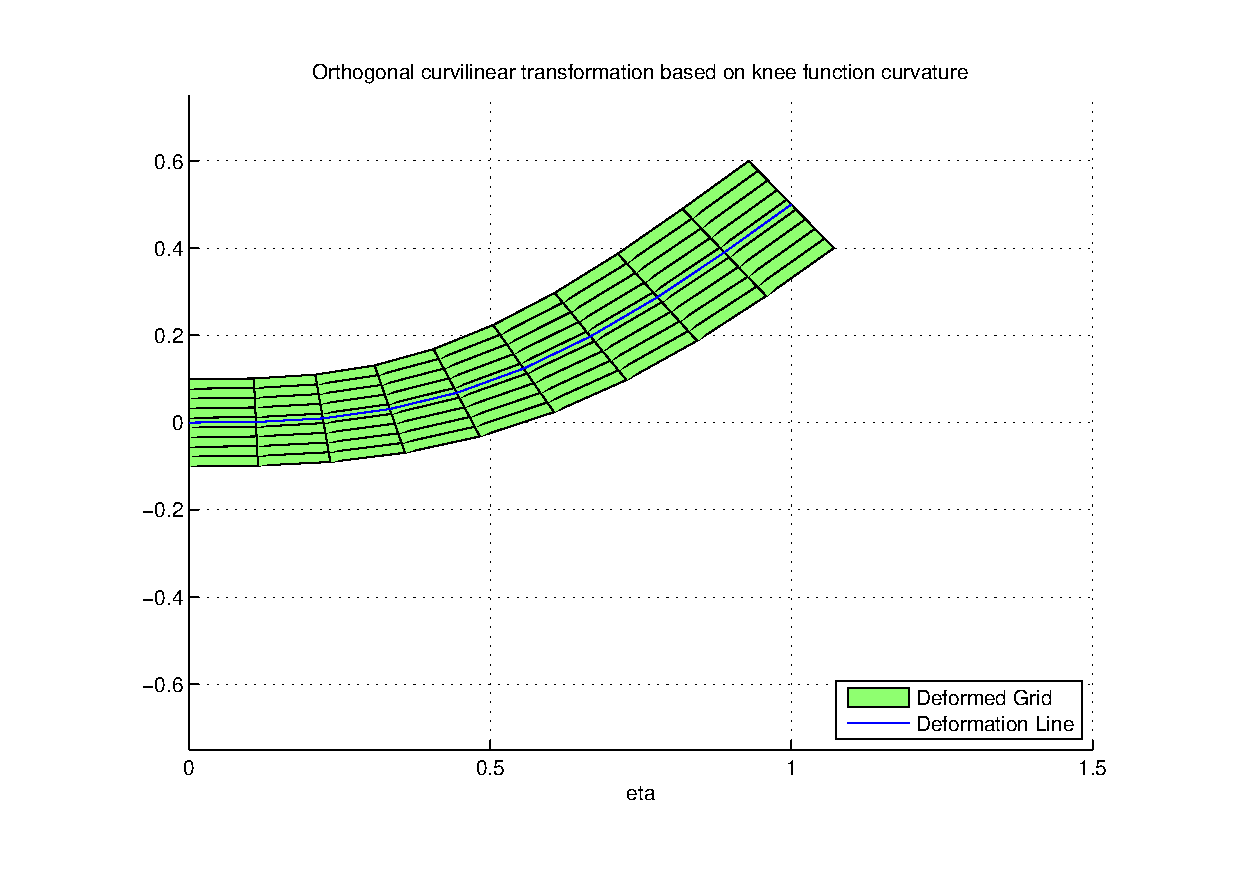
\includegraphics[width=0.9\textwidth]{fig/deformed_grid} 

\caption{An orthogonal curvilienear transformation defined from the g-eta knee
function curvature primitive in eta \emph{(not renormalized) \label{fig:An-orthogonal-curvilienear}}}
\end{figure}



\subsection{Scaling the smooth knee function}

We recall the definition of the $\eta$ coordinate transformation
to write its jacobian
\[
\frac{\partial\eta}{\partial x}=\frac{1}{2\delta}
\]


so that we can state the dimensional $p$ function and its $1^{st}$
derivative in terms of $g's$ derivatives:
\[
p_{\left(x\right)}=2\delta mg_{\left(\eta_{\left(x\right)}\right)}+c
\]


\[
\frac{\partial p}{\partial x}=\frac{\partial p}{\partial\eta}\frac{\partial\eta}{\partial x}=2\delta m\frac{\partial g}{\partial\eta}\frac{1}{2\delta}=m\frac{\partial g}{\partial\eta}\qquad,\quad m,\delta\perp x,\eta
\]


and for the $2^{nd}$ derivative we get:
\[
\frac{\partial^{2}p}{\partial x^{2}}=\frac{\partial}{\partial x}\left(m\frac{\partial g}{\partial\eta}\right)=m\frac{\partial}{\partial x}\left(\frac{\partial g}{\partial\eta}\right)=m\frac{\partial^{2}g}{\partial\eta^{2}}\frac{\partial\eta}{\partial x}
\]
\[
=\frac{m}{2\delta}\frac{\partial^{2}g}{\partial\eta^{2}}=\frac{m}{2\delta}\left(6\eta-6\eta^{2}\right)
\]


So the curvature of the $p-x$ graphline will be given as:
\[
\kappa_{\left(x\right)}^{p}=\frac{\frac{\partial^{2}p}{\partial x^{2}}}{\left(1+\left(\frac{\partial p}{\partial x}\right)^{2}\right)^{\frac{3}{2}}}=\frac{\frac{m}{2\delta}\frac{\partial^{2}g}{\partial\eta^{2}}}{\left(1+\left(m\frac{\partial g}{\partial\eta}\right)^{2}\right)^{\frac{3}{2}}}=\frac{1}{2\delta}\frac{m\frac{\partial^{2}g}{\partial\eta^{2}}}{\left(1+\left(m\frac{\partial g}{\partial\eta}\right)^{2}\right)^{\frac{3}{2}}}
\]
\[
=\frac{1}{2\delta}\frac{m\left(6\eta-6\eta^{2}\right)}{\left(m^{2}\left(3\eta^{2}-2\eta^{3}\right)^{2}+1\right)^{\frac{3}{2}}}
\]


Before we take the $x$ primitive of $\kappa_{p}$ we observe that:
\[
d\eta=d\left(\frac{x-x_{1}}{2\delta}\right)=\frac{dx}{2\delta}\quad\Leftrightarrow\quad dx=2\delta d\eta
\]


So that we can write:
\[
K_{\left(x\right)}^{p}=\int\kappa^{p}dx=\int\kappa^{p}2\delta d\eta=\int\frac{1}{2\delta}\frac{m\frac{\partial^{2}g}{\partial\eta^{2}}}{\left(1+\left(m\frac{\partial g}{\partial\eta}\right)^{2}\right)^{\frac{3}{2}}}2\delta d\eta=\int\frac{m\frac{\partial^{2}g}{\partial\eta^{2}}}{\left(1+\left(m\frac{\partial g}{\partial\eta}\right)^{2}\right)^{\frac{3}{2}}}d\eta
\]


and find an analytical primitive%
\footnote{With the symbolic toolbox!%
}:
\[
K_{\left(x\right)}^{p}=\int\kappa^{p}dx=\frac{m\left(3\eta^{2}-2\eta^{3}\right)\sqrt{m^{2}\left(3\eta^{2}-2\eta^{3}\right)^{2}+1}}{4m^{2}\eta^{6}-12m^{2}\eta^{5}+9m^{2}\eta^{4}+1}+C_{kp}\qquad,\quad\eta=\eta_{\left(x\right)}
\]



\subsection{The smoothed hinge line deformation function}

Following our definition for the smoothed hinge line deformation function
$f\in C^{2}$ we can write:
\[
f_{\left(x\right)}=\begin{cases}
c & \quad,\quad x<x_{h}-\delta\\
2\delta mg_{\left(\eta_{\left(x\right)}\right)}+c & \quad,\quad x_{h}-\delta\leq x<x_{h}+\delta\\
c+m\left(x-x_{hinge}\right) & \quad,\quad x_{h}+\delta\leq x
\end{cases}
\]


together with its first derivative:
\[
\frac{df}{dx}=\begin{cases}
0 & \quad,\quad x<x_{h}-\delta\\
m\left.\frac{\partial g}{\partial\eta}\right|_{\eta_{\left(x\right)}} & \quad,\quad x_{h}-\delta\leq x<x_{h}+\delta\\
m & \quad,\quad x_{h}+\delta\leq x
\end{cases}
\]


and its second derivative:
\[
\frac{d^{2}f}{dx}=\begin{cases}
0 & \quad,\quad x<x_{h}-\delta\\
\frac{m}{2\delta}\left.\frac{\partial^{2}g}{\partial\eta^{2}}\right|_{\eta_{\left(x\right)}} & \quad,\quad x_{h}-\delta\leq x<x_{h}+\delta\\
0 & \quad,\quad x_{h}+\delta\leq x
\end{cases}
\]


which implies that the curvate of the $f-x$ line will be null everywhere
except in the $\left[x_{h}-\delta\,,\, x_{h}+\delta\right]$ interval,
so that we can write:
\[
\kappa_{\left(x\right)}^{f}=\begin{cases}
0 & \quad,\quad x<x_{h}-\delta\\
\kappa_{\left(x\right)}^{p} & \quad,\quad x_{h}-\delta\leq x<x_{h}+\delta\\
0 & \quad,\quad x_{h}+\delta\leq x
\end{cases}
\]


which therefore admits a straightforward analytical primitive:
\[
K_{\left(x\right)}^{f}=\begin{cases}
0 & \quad,\quad x<x_{h}-\delta\\
K_{\left(x\right)}^{p} & \quad,\quad x_{h}-\delta\leq x<x_{h}+\delta\\
K_{\left(x_{h}+\delta\right)}^{p} & \quad,\quad x_{h}+\delta\leq x
\end{cases}
\]


where the constant $C_{kp}$ of the $K_{\left(x\right)}^{p}$ function
will be chosen such that:
\[
K_{\left(x_{h}-\delta\right)}^{p}=0
\]


whereby we can write

\[
\eta_{\left(x_{h}-\delta\right)}=0\quad\Rightarrow\quad K_{\left(x_{h}-\delta\right)}^{p}=0+C_{kp}\quad\Rightarrow\quad C_{kp}=0
\]


so $K^{p}$ is explicitly written as:
\[
K_{\left(x\right)}^{p}=\frac{m\left(3\eta^{2}-2\eta^{3}\right)\sqrt{m^{2}\left(3\eta^{2}-2\eta^{3}\right)^{2}+1}}{4m^{2}\eta^{6}-12m^{2}\eta^{5}+9m^{2}\eta^{4}+1}\qquad,\quad\eta=\eta_{\left(x\right)}
\]



\section{The Orthogonal Curvilinear Transformation }

We follow Goldstein (1938) in our exploration of Lam�'s (1859) formidable
work on curvilinear coordinate systems, to define a transformation:
\[
T:\left(x,y\right)\rightarrow\left(s,n\right)
\]


from it's Jacobian:

\[
ds=h_{1}dx\qquad,\qquad dn=h_{2}dy
\]
\[
\left[\begin{array}{c}
ds\\
dn
\end{array}\right]=\left[\begin{array}{cc}
h_{1} & 0\\
0 & h_{2}
\end{array}\right]\left[\begin{array}{c}
dx\\
dy
\end{array}\right]
\]


with the $h$ functions given in terms of the reference line curvature:
\[
h_{1}=h_{1\left(x\right)}=1+\kappa y\qquad\qquad h_{2}=1
\]


We will now try to find an explicit expression for the transformation
$T$ by integrating the above definition in terms of differential
elements. This is easier for the second coordinate so that is where
we will start to illustrate the procedure:
\[
n=\int dn=\int h_{2}dy\qquad\Rightarrow n=y+C_{yn}
\]


where $C_{yn}$is a constant such that:
\[
\left(n=0\Leftrightarrow y=0\right)\quad\Rightarrow\quad C_{yn}=0\quad\Rightarrow\quad n=y
\]


And we are now ready to attack the first coordinate:
\[
ds=h_{1}dx=\left(1+\kappa y\right)dx\quad\Leftrightarrow\quad\int ds=\int\left(1+\kappa y\right)dx
\]
\[
\Leftrightarrow\quad s=x+y\int\kappa dx\qquad,\quad y\perp x
\]


Defining 
\[
K_{\left(x\right)}=\int\kappa dx
\]


we can write: 
\[
s_{\left(x,y\right)}=x+yK_{\left(x\right)}
\]


So the $T$ transformation can be written as:
\[
\left[\begin{array}{c}
s\\
n
\end{array}\right]\equiv T_{\left(x,y\right)}=\left[\begin{array}{c}
x+yK_{\left(x\right)}\\
y
\end{array}\right]
\]



\subsection{For the particular case of a flapped airfoil}

In this case we can use the expression for $K_{\left(x\right)}^{f}$
of the deformed hingeline:
\[
K_{\left(x\right)}^{f}=\begin{cases}
0 & \quad,\quad x<x_{h}-\delta\\
K_{\left(x\right)}^{p} & \quad,\quad x_{h}-\delta\leq x<x_{h}+\delta\\
K_{\left(x_{h}+\delta\right)}^{p} & \quad,\quad x_{h}+\delta\leq x
\end{cases}
\]


where

\[
K_{\left(x\right)}^{p}=\frac{m\left(3\eta^{2}-2\eta^{3}\right)\sqrt{m^{2}\left(3\eta^{2}-2\eta^{3}\right)^{2}+1}}{4m^{2}\eta^{6}-12m^{2}\eta^{5}+9m^{2}\eta^{4}+1}\qquad,\quad\eta=\eta_{\left(x\right)}
\]
\[
\eta_{\left(x\right)}=\frac{x-x_{h}}{2\delta}+\frac{1}{2}\qquad,\qquad m=\tan\theta\qquad,\qquad\delta=\mbox{chosen!}
\]


Which provides an effective way to deform airfoil shapes and meshes
to account for airfoil flapping, as shown on figure \ref{fig:Original-and-Deformed},
generated with our first code implementation, which is fully vectorized,
and therefore fast for a Matlab code.

\begin{figure}
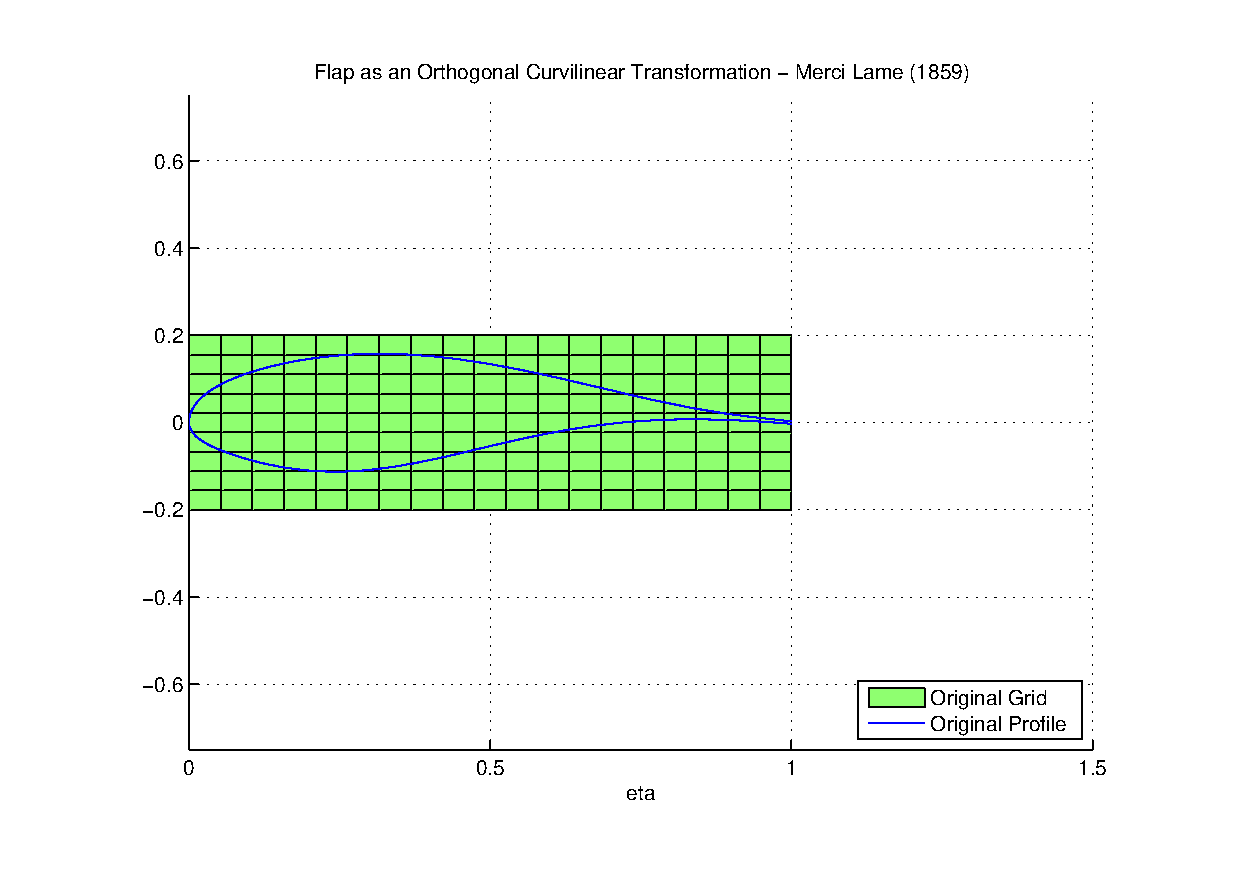
\includegraphics[width=0.9\textwidth]{fig/original_airfoil_on_grid}

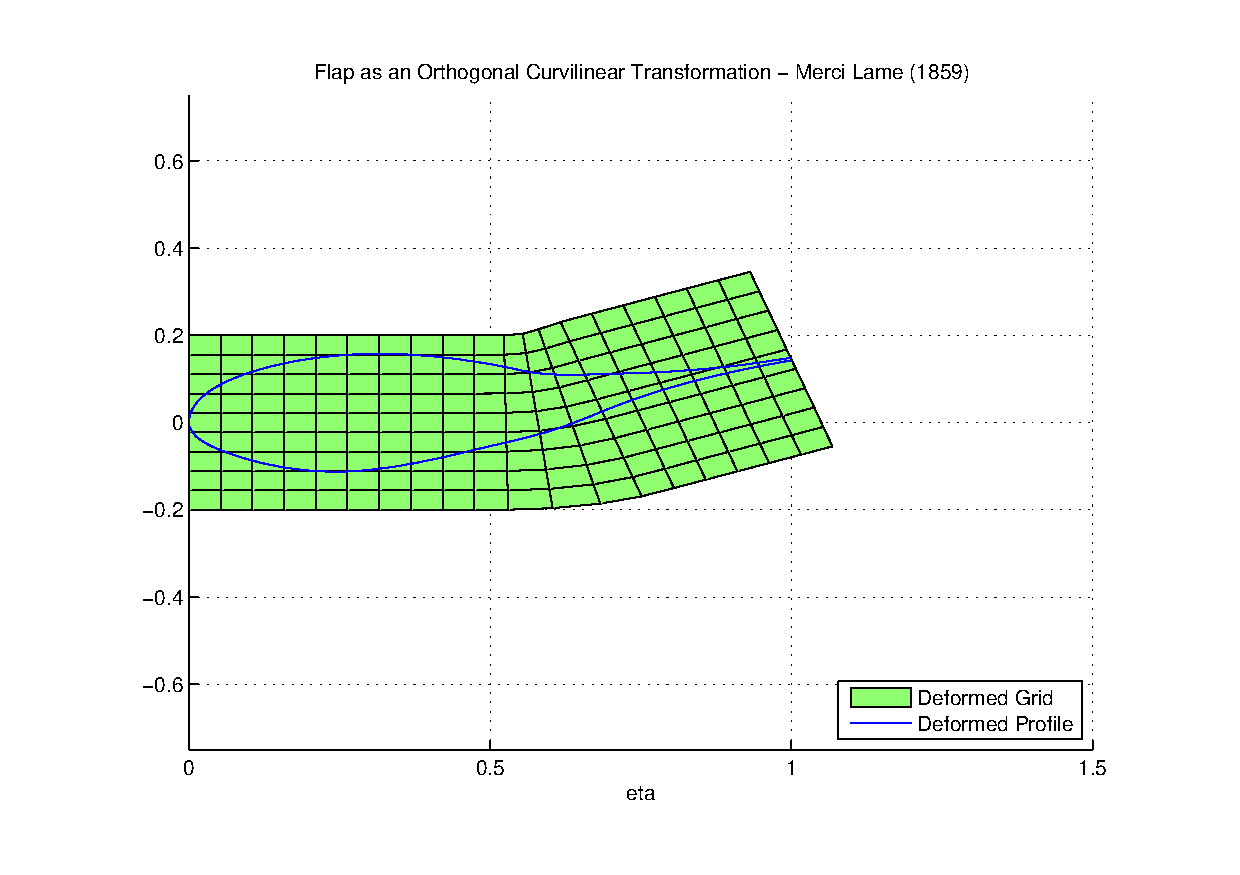
\includegraphics[width=0.9\textwidth]{fig/deformed_airfoil_on_grid}

\caption{Original and Deformed airfoils on Mesh (not renormalized, purely afine
transformation)\label{fig:Original-and-Deformed}}
\end{figure}



\subsection{Towards a general approach}

In general, the curvature of a graph line for any function $f$ is
written as:
\[
\kappa_{g}=\frac{\frac{\partial^{2}f}{\partial x^{2}}}{\left(1+\left(\frac{\partial f}{\partial x}\right)^{2}\right)^{\frac{3}{2}}}
\]


and this expression has a general primitive in $x$ given as%
\footnote{Computed with Wolfram Alpha, even though it would not be impossible
to see it by hand!%
}:
\[
K=\int\kappa dx=\int\frac{\frac{\partial^{2}f}{\partial x^{2}}}{\left(1+\left(\frac{\partial f}{\partial x}\right)^{2}\right)^{\frac{3}{2}}}dx=\frac{\frac{\partial f}{\partial x}}{\left(1+\left(\frac{\partial f}{\partial x}\right)^{2}\right)^{\frac{1}{2}}}+C
\]


And this opens many possibilities, namely to calculate transformations
along arbitrarly defined $C^{2}$ continuous lines for which we have
the first and second derivatives%
\footnote{In fact, the 1st derivative will be sufficient whenever the constant
can be calculated otherwise, for example by matching two points of
the T transformation.%
}.

In fact, arbitrary deformations can be defined based on a set of points
describing an arbitraty.


\section{Renormalizing the Hinge Line}

The hinge line depicted in figure \ref{fig:An-orthogonal-curvilienear}
does not have the same lenght as the original hingeline. However,
on a real flapping airfoil the hinge line retains its lenght and the
chord may change slightly %
\footnote{if we define it as the distance from the trailing edge to the leading
edge, which becomes debatable!%
}.

It is therefore desirable to enhance our transformation by renormalizing
the hinge line. Our last code implementation incorporates an approximate
renormalization of the hinge line, and the details are described in
the code comments. 

The current implementation is very simple, but has some limitations
from an analytical standpoint:
\begin{itemize}
\item The purely affine character is lost, but the renormalized transformation
remains quasi afine
\item The renormalized transformation introduces a single 2nd derivative
discontinuitie at the hinge point.
\end{itemize}
As such, that the current implementation is only accurate for moderate
flap angles:
\begin{enumerate}
\item Errors are negligible at 10degrees
\item Noticeable but small at 20degrees
\item Relevant at 45 degrees
\end{enumerate}
A generalized, fully $C^{2}$ version valid for large flapping angles
may could be developped later. We have ideas on how to do that while
implementing an adaptative smoothing parameter to deal with very thick
airfoils, but that did not seem necessary at this stage. 

\begin{figure}
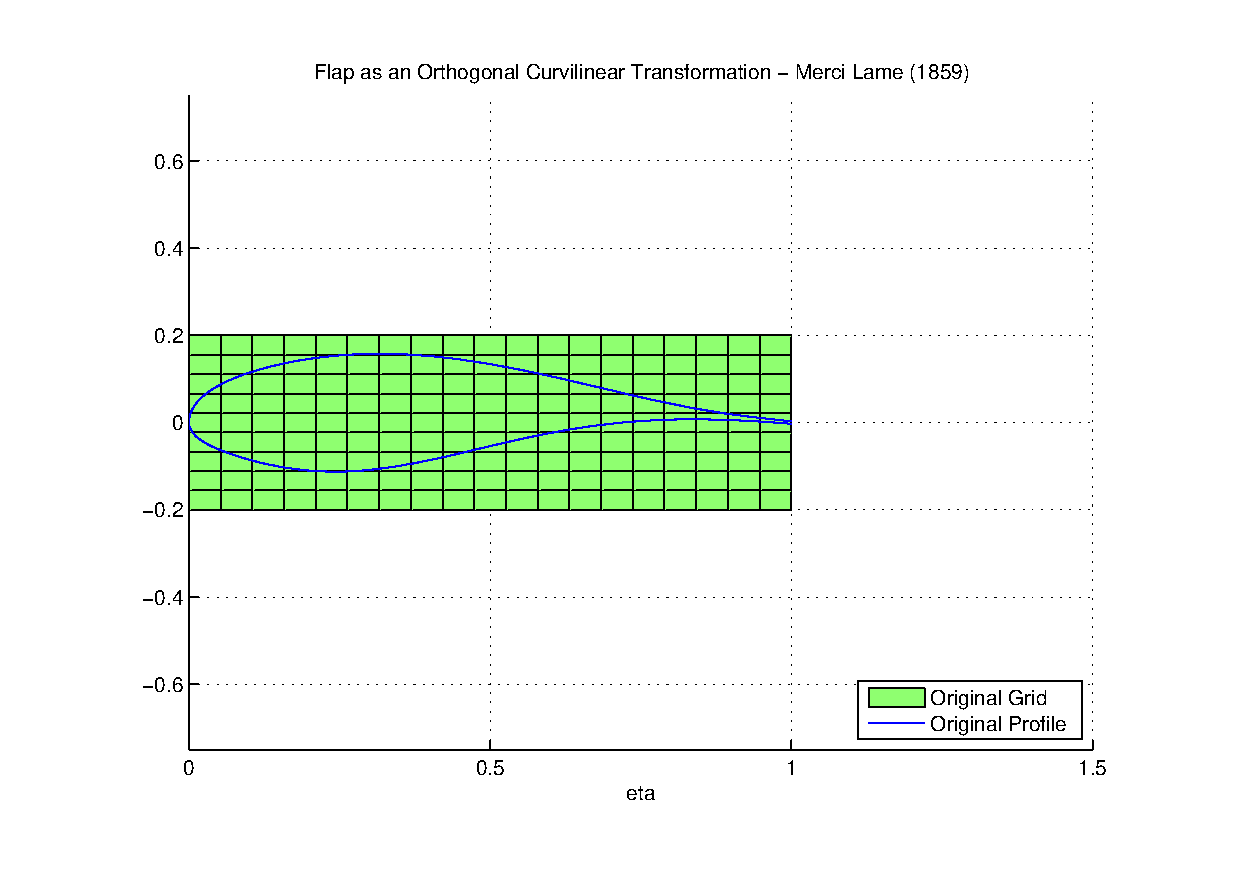
\includegraphics[width=0.9\textwidth]{fig/original_airfoil_on_grid}

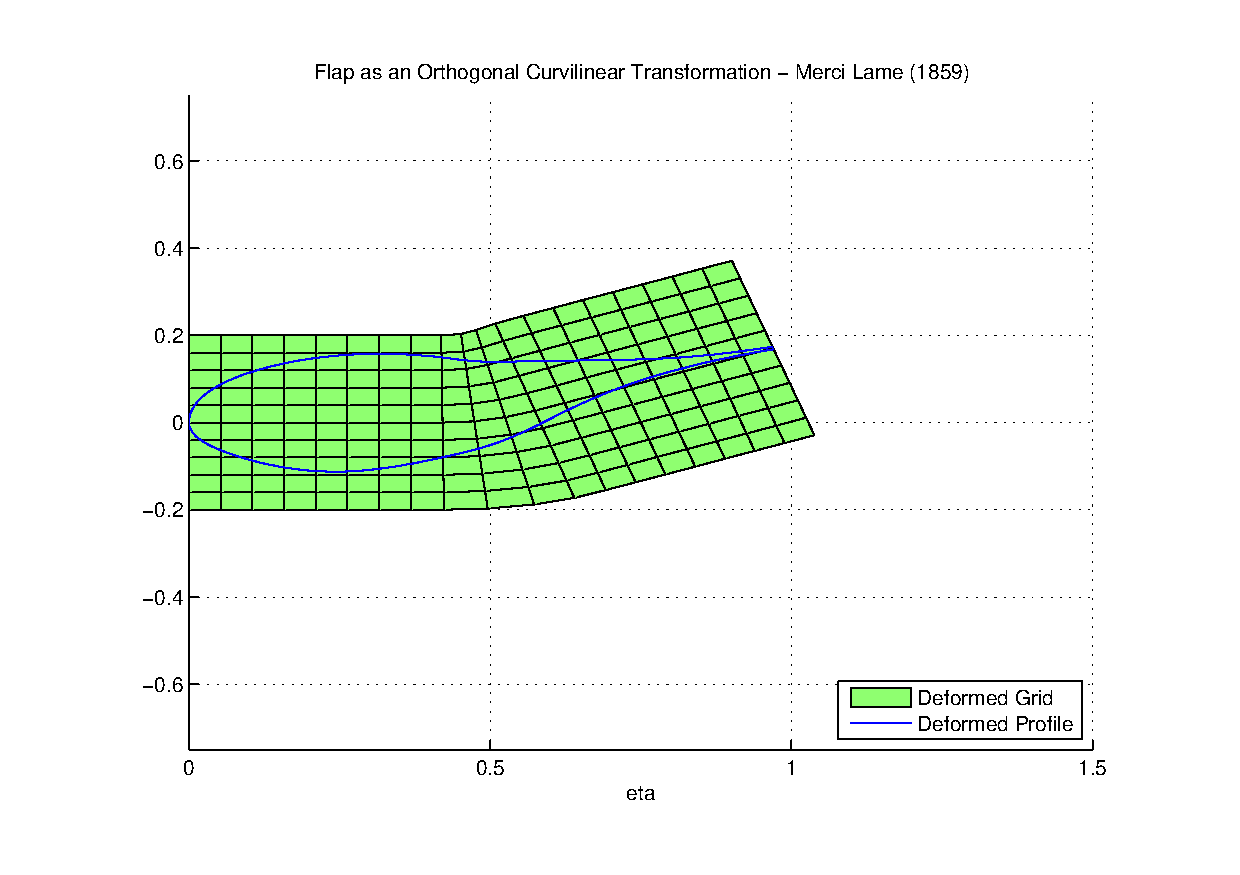
\includegraphics[width=0.9\textwidth]{fig/deformed_airfoil_on_grid_renormalized}

\caption{Original and Deformed airfoils on Mesh (not renormalized, purely afine
transformation)\label{fig:Original-and-Deformed-renormalized}}
\end{figure}


\begin{figure}
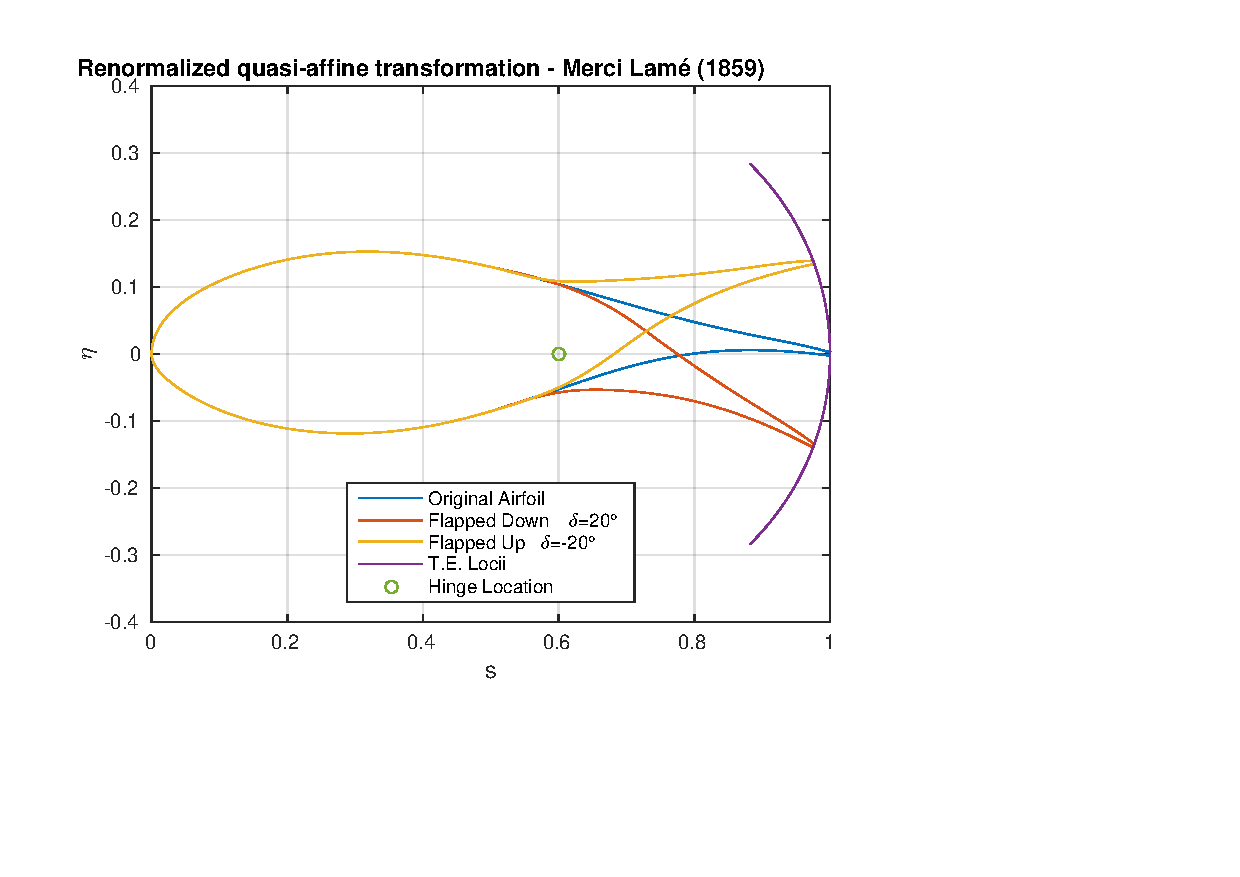
\includegraphics[bb=0bp 80bp 445bp 421bp,clip,width=0.9\linewidth]{fig/renormalized_airfoil_flapping}

\caption{Renormalized Quasi Affine Flapping Airfoil Transformation, a practical
example \label{fig:Renormalized-Quasi-Affine}}
\end{figure}


Figures \ref{fig:Original-and-Deformed-renormalized} and \ref{fig:Renormalized-Quasi-Affine}
show the the renormalized transformation. The circle of figure \ref{fig:Renormalized-Quasi-Affine}
highlights that the Trailing Edge position moves in the same way as
it would with a real flap, because the lenght of the total chordline
is preserved. 

The purely afine transformation did not preserve this important feature,
nor the smooth transformations that are currently in use!
\end{document}
